



%----------------------------------------------------------------------------------------

\newpage

\section[Interaction model][Modèle d'interaction]{Dynamical extension of the interaction model}{Extension dynamique du modèle d'interaction}





%----------------------------------------------------------------------------------------

%%%%%%%%%%%%%%%%%
\subsection{Macroscopic Model of Co-evolution}{Modèle macroscopique de co-évolution}


%%%%%%%%%%%%%%%%%
\subsubsection{Rationale}{Hypothèses et choix de modélisation}

% abstract conf Guangzhou

% The complexity of Urban Systems is closely linked to the co-evolutive character of their different components or agents (Pumain, 1997). In the case of cities and transportation networks, this co-evolution has been shown empirically (Bretagnolle, 2007) but remains poorly understood in terms of its dynamical processes. We introduce a model of spatial interactions between cities at the macro-scale, in the spirit of stochastic urban growth models inheriting from the Gibrat model (Favaro and Pumain, 2011). We include evolving transportation networks, in order to explore stylized hypothesis on the interactions and drivers of the growth of both network and cities. In a multi-modeling fashion, the model can take into account various processes such as between cities direct interactions, network-mediated interactions, feedback of network flows, and for the network demand-induced growth. The latter is tested at different abstraction levels that are the time-distance matrix between cities, and physical network growth trying to satisfy greedy time-gain optimization criteria. We use as a benchmark network the geographical shortest paths that have been shown in a previous work to already capture network effects (Raimbault, 2016). The model is tested and explored on synthetic city systems, generated following a simple heuristic to follow the rank-size law and Central Place Theory. The systematic exploration through intensive computation unveils different interaction regimes accross the parameter space. In some, the introduction of the network can drastically change the fate of some cities, whereas the top-distribution hierarchy is reinforced, what is consistent with empirical observations in the literature. Some regimes actually exhibit circular causalities between network and city growth, corresponding to the intricated co-evolution. The model will be applied to the French Urban System on long time dynamical data (Pumain-INED database for populations spanning between 1831 and 1999, with the evolving railway network from 1850 to 2000, and a specifically-designed database of the highway networks containing its full genesis from 1950 to 2015), and to the Chinese Urban System after 2000 with the High Speed Rail (HSR) network, both realized and planned. Expected results concern both accurate city population growth reproduction, and network patterns, i.e. how does taking into account dynamical networks can introduce further exploratory power in such models, and reciprocally how can such coupled models produce realistic networks compared to more classical autonomous models of network growth. The role of medium-sized cities on the trajectories of the system can also be examined with the model. Finally, a comparison between the urban systems in different geographical and political contexts and at different scales should unveil implications of planning on the interactions between networks and cities, for example by comparing the rather bottom-up growth of the French railway network to the top-down state-planned French highway and Chinese HSR networks.


Cette première approche se place dans une logique d'extension directe du modèle d'interactions au sein d'un système de villes présenté en chapitre~\autoref{ch:evolutive}, c'est à dire à une échelle macroscopique et avec une ontologie typique au systèmes de villes. Toujours dans un choix de simplicité, dont la relaxation sera explorée pour le cas d'application à la Chine avec l'ajout de variables économiques, nous restons ici à une description uni-dimensionelle des villes par leur population. Concernant la croissance du réseau, nous proposons de se placer également à un niveau relativement agrégé et simplifié, en testant des heuristiques de croissance répondant à une demande, à différents niveaux d'abstraction. 







%%%%%%%%%%%%%%%%%
\subsubsection{General Formulation}{Formulation Générique}




%%%%%%%%%%%%%%%%%
\begin{figure}
\centering
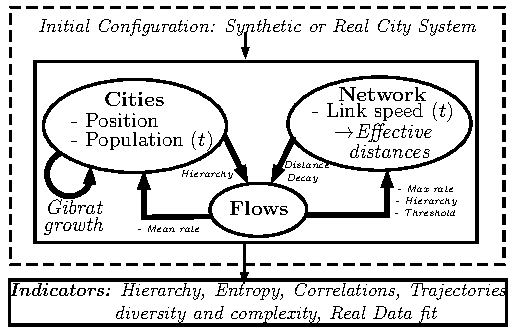
\includegraphics[width=\textwidth]{Figures/MacroCoEvolModel/model}
\caption[][Schématisation du modèle]{}{Représentation abstraite des processus du modèle.}
\end{figure}
%%%%%%%%%%%%%%%%%








%%%%%%%%%%%%%%%%%
\subsection{Application to Synthetic Data}{Application à des Données Synthétiques}

%%
% Implementation architecture : scala/oml extension wrapper ? simpler to do full-netlogo : comment on that (//simfamily etc)
%  Interactions (Matrix-based) <-> Network





%%%%%%%%%%%%%%%%%
\subsection[Applications][Applications]{Applications to Case Studies}{Applications à des cas d'étude}


\subsubsection{}{Système de Villes Français}

\paragraph{}{Données de Réseau}

% description de la base Thévenin pour le train ; et de la base autoroutes ("data paper" en annexe -> penser à faire un vrai data paper avec Florent.)


\todo{Questions concrètes à poser au modèle, expériences ciblées : (i) le modèle calibre-t-il mieux les populations (en prenant en compte les paramètres supplémentaires) ; (ii) le modèle produit-il des formes de réseau crédibles ? ; (iii) éventuellement si les correlations temporelles sont calculées sur les vrais données, le modèle peut-il être calibré au second ordre (sur les correlations/causalités) ?}


\comment[JR]{attention, expliquer le choix des indicateurs de réseau, il faut qu'ils soient adaptés à l'échelle : cf Mimeur nombre d'intersection - relève un peu de la modélisation procédurale.}

\comment{\cite{mimeur:tel-01451164} la thèse de Mimeur est un pont intéressant entre géographie et approches éco de Levinson (modèle de croissance type slime mould ?). plus fait des stats spatiales pour lier croissance pop et accessibilité : checker si même résulats quand fera spatio-temp causalities sur réseau ferré et autoroutier et croissance pop. remarque : trucs bizzares, essaie d'expliquer pour petites villes, mais pas approprié, pb du choix de l'échelle, de ce qui est du bruit et du signal - semble tout mélanger : importance du preprocessing et traitement du signal (cf correlations des taux de croissance). Tester effets fixes régions/départements ? fait GWR finalement ?}













